\documentclass{svproc}
%
\usepackage{graphicx}%
\usepackage{multirow}%
\usepackage{amsmath,amssymb,amsfonts}%
\usepackage{mathrsfs}%
\usepackage[title]{appendix}%
\usepackage{xcolor}%
\usepackage{textcomp}%
\usepackage{manyfoot}%
\usepackage{booktabs}%
\usepackage{algorithm}%
\usepackage{algorithmicx}%
\usepackage{algpseudocode}%
\usepackage{listings}%
\usepackage{url}
\def\UrlFont{\rmfamily}

\renewcommand{\topfraction}{.99}
\renewcommand{\dbltopfraction}{.99}
\renewcommand{\bottomfraction}{.99}
\renewcommand{\textfraction}{.01}
\renewcommand{\floatpagefraction}{0.9}
\renewcommand{\dblfloatpagefraction}{0.9}

\usepackage[normalem]{ulem}
\usepackage{bm}
\usepackage{xspace}
\usepackage{subcaption}

\usepackage{color}
\def\green#1{\textcolor[rgb]{0,0.6,0}{#1}}
\def\black#1{\textcolor[rgb]{0,0,0}{#1}}
\def\dgreen#1{\textcolor[rgb]{0.02,0.50,0.05}{#1}}
\def\gray#1{\textcolor[rgb]{0.5,0.5,0.7}{#1}}
\def\red#1{\textcolor{red}{#1}}
\def\blue#1{\textcolor{blue}{#1}}
\def\Blue{\color[rgb]{0,0,1}}
\def\Red{\color[rgb]{1,0,0}}
\def\Dgreen{\color[rgb]{0.02,0.55,0.04}}
\def\Black{\color[rgb]{0,0,0}}
\def\ignore#1{}

\usepackage[normalem]{ulem}
\usepackage{bm}
\usepackage{booktabs}
\usepackage{xspace}
\usepackage{subcaption}

% track-changes helpers (kept from last year's setup)
\newcommand{\add}[1]{\textcolor{blue}{#1}}
\newcommand{\erase}[1]{\textcolor{red}{\sout{#1}}}
\def\subst#1#2{\add{#1}{ \erase{#2}}}

% parameters definition (same convention as docs/journal.tex)
\def\post{\rho}                 % posting probability
\def\BoundedConfidence{\epsilon} % bounded confidence (rejection) threshold
\def\feed{F}                    % feed
\def\Stubbornness{\mu}           % stubbornness
\def\maxfollower{S_{\it fol}}    % max followee capacity
\def\maxfeed{S_{\it fd}}         % feed capacity
\def\VCR{\kappa}                 % vocal comfort radius (expression threshold)

\begin{document}
\mainmatter

\title{When Do Moderate Hubs Amplify Extreme Opinion Activation? \\ A Two-Layer Homophily Mechanism in Adaptive Social Networks}
\titlerunning{Moderate Hubs and Two-Layer Homophily}

\author{Tomoya Takeda\inst{1}, Fujio Toriumi\inst{2}, Toshiharu Sugawara\inst{1}}
\authorrunning{Tomoya Takeda, Fujio Toriumi and Toshiharu Sugawara} % abbreviated author list (for running head)

\institute{Department of Computer Science and Communications Engineering,
\\Waseda University, 3-4-1 Okubo, Shinjyuku-ku, 169-8555, Tokyo, Japan.\\
\email{tomoya.leo9@fuji.waseda.jp}, \email{sugawara@waseda.jp}
\and
Department of Systems Innovation, The University of Tokyo, \\7-3-1
Hongo, Bunkyo-ku, 113-8656, Tokyo, Japan.\\
\email{tori@sys.t.u-tokyo.ac.jp}
}

\maketitle

\begin{abstract}\Blue
With the rapid expansion of web communication platforms, hub users
have become critical actors in online opinion expression dynamics;
however, their effects on polarized posting behavior remain poorly
understood. Using an agent-based model on heavy-tailed adaptive social
networks, we study how moderately positioned hubs shape
opinion-sharing behavior. Across a comprehensive suite of experiments,
we observe a consistent pattern in which active moderate hubs boost
moderate-camp posting while suppressing near-extreme posting. Their
influence on the ideologically distant extreme camp, however, is
highly complex: moderate hubs can act as mediators or facilitators of
activation depending on network conditions. We trace this regime shift
to a two-layer homophily mechanism, structural and perceptual, which
determines whether the two camps are perceived as one group
(mediation) or as separate communities (facilitation). Moderate hubs
are therefore not universally stabilizing bridges; their brokerage
role flips between mediation and facilitation depending on how
homophilic the two camps are perceived to be.
\Black
\keywords{Social networks, Opinion dynamics, Agent-based simulation,
  Social media, Computational Social Science} 
\end{abstract}

\Blue


\section{Introduction}\label{sec:intro}
Social media and web communication platforms have become the primary
venues for various styles of speech and discussion, rather than merely
for sharing individual ideas, thereby exerting a significant effect on
public opinion formation. Unlike traditional face-to-face
communication, hub users or influencers --- followed by a large number
of users --- can create posts that are disproportionately amplified
across a platform's population, giving them immense influence on a
given opinion environment. The role and effect of these hubs have been
well studied through agent-based simulation and data mining,
particularly from the perspective of information diffusion. However,
their effects on polarized, controversial opinion dynamics are not yet
fully understood, specifically regarding moderately positioned hubs as
opposed to strongly identified opinion leaders.
\par


Therefore, we investigate how the sharing activity of these moderate
hubs affects polarized opinion dynamics. Using an agent-based
simulation on heavy-tailed adaptive social networks, we find that
active moderate hubs do not uniformly mediate extreme-camp posting:
they consistently boost posting activity among aligned moderate users
while suppressing that of the ideologically nearby near-extreme camp,
but their effect on the ideologically distant extreme camp is
conditional. The results show that this conditional effect manifests
as a clear regime shift governed by perceptual and structural
parameters.
\par


Although mechanistically distinct, the effects of these two parameters
appear to converge on a single, unifying homophily logic: when the
near-extreme and extreme camps are effectively perceived as one
homogeneous group, suppressing near-extreme posting also mediates
extreme-camp activity. When they are instead perceived as separate,
distinct communities, moderate hubs' suppression of near-extreme
posting does not reach the extreme camp. Instead, it isolates the
extreme camp into a more pure, self-contained echo chamber, which
facilitates, rather than dampens, its activation. This perception of
homophily versus heterophily is governed by two distinct layers: a
perceptual layer, defined by how wide an opinion difference users find
comfortable to engage with, which determines whether reached content
registers as similar enough to elicit participation; and a structural
layer, defined by how readily agents disconnect from ties they no
longer tolerate, which shifts the threshold of opinion difference that
must be tolerated for the two camps to be treated as a single group.
\par

%
\Black%%{}######
%

%[How these two layers relate to one another]

The role of bridge nodes, or brokers, has long been studied, yet its
effect on social media remains highly complex due to the varied
dynamics such platforms exhibit.This study offers a novel, mechanistic
account of the conditional role of brokerage nodes.


\section{Related Work}\label{sec:related}
Social networks have long been studied as static structures, most
notably in seminal work on small-world topology~\cite{watts1998};
more recently, however, they have also been modeled as systems whose
topology coevolves with the opinions and behaviors of the individuals
embedded in them.
Building on the classic Voter model~\cite{clifford1973}, Vazquez et
al.~\cite{vazquez2008} used an \emph{agent-based model (ABM)} to analyze
coevolutionary dynamics based on two coupled rules -- state updating
and edge rewiring -- revealing a phase transition between connected
and fragmented networks governed by degree settings.
Opinion dynamics is one of the major fields where this style of
coevolving-network model has been fruitfully applied: Kozma and
Barrat~\cite{kozma2008} modeled how agents adaptively rewire their
social ties in response to disagreement, showing the dominant effect
of homophilic rewiring on the resulting network structure. This
coevolving-network model builds on \emph{bounded confidence},
formalized by Deffuant et al.~\cite{deffuant2000} and Hegselmann and
Krause~\cite{hegselmann2002}, in which an agent updates its opinion
only by averaging with others whose opinion falls within a fixed
tolerance window.
With the precipitous proliferation of social media in recent years,
our public discourse has been altered significantly from traditional
face-to-face communication, and in line with this homophilic-rewiring
mechanism, Sasahara et al.~\cite{sasahara2020} used an ABM to
confirm that social influence combined with the unfollowing
process successfully reproduces the politically polarized follow
network observed in real-world social media data~\cite{conover2011}.

Whether such bridging roles are inherently stabilizing, 
however, is far from settled in the context of social media.
Classic network theory established that ties bridging otherwise
disconnected communities act as a source of connectivity and
innovation rather than redundancy, whether characterized as
\emph{weak ties} diffusing influence and information across group
boundaries~\cite{granovetter1973} or as \emph{broker} nodes spanning
structural holes~\cite{burt1992}, a bridging role later quantified as
\emph{betweenness centrality}, the count of shortest paths between any
two nodes in a network that pass through a given node~\cite{freeman1977}.
On social media, however, this integrative reading does not hold
unconditionally: Cha et
al.~\cite{cha2010} observed that highly-followed users do not
necessarily exert larger influence, an important caveat for influence
maximization in social media marketing, and subsequent ABM studies
found a hub's effect on the surrounding population to be conditional
rather than uniformly integrative. Using an ABM, Helfmann et
al.~\cite{helfm2023} showed that hub users who adopt extreme attitudes
can gain more followers on social media. Also with an ABM, Betts et
al.~\cite{betts2023} found that,
unlike an extremist influencer whose activity always accelerates
polarization, a neutral influencer's effect on polarization inverts
depending on its own tolerance for disagreeing views -- that is,
brokerage by a moderate hub is not necessarily stabilizing.

As reviewed above, most of these studies take opinion position itself
as the outcome, whether an influencer's own attitude~\cite{helfm2023}
or a population's aggregate polarization~\cite{betts2023,sasahara2020}.
On social media, however, influence operates not only through changes
in private opinion but also through the decision to express or
withhold it. Following the \emph{spiral-of-silence} tradition, in
which individuals modulate whether they voice an opinion according to
their perceived opinion climate~\cite{noelle-neumann1974},
Krassa~\cite{krassa1988} used an ABM to test this dynamic through
social groups and selective perception. Even simulation-based studies
focusing on social media, however, tend to treat opinion position as
the primary outcome, leaving expression secondary. We therefore take
posting, or vocality, as our outcome throughout, investigating in
particular whether and under what conditions moderate hubs'
ostensibly mediating role produces complex effects on opinion
expression across groups, using agent-based simulation.



\section{Model}\label{sec:model}

\subsection{Agent-Based Model}\label{sec:model-abm}

We simulate opinion and posting dynamics on a directed 
graph $G=(A,E)$, where $A=\{1,2,\dots,N\}$ is the set 
of $N$ agents representing individual social media 
users and $E\subseteq A\times A$ is the set of 
directed follow edges, so that $(i,j)\in E$ means
agent $i$ follows agent $j$, with a corresponding
adjacency matrix $A$ such that
$A_{ij}=1$ if $(i,j)\in E$ and $A_{ij}=0$ otherwise.
This follow graph evolves through the social media
behaviors introduced in
Section~\ref{sec:model-behaviors}.
The dynamics proceed in discrete time 
steps $t\in\{0,1,2,\dots\}$.
Each agent $i\in A$ holds an opinion $O_i(t)\in[-1,1]$,
representing its stance on a single controversial
issue at time $t$; the boundaries $-1$ and $1$
denote the two most extreme opposing positions,
and $0$ denotes a moderate or neutral stance.
Hereafter, we group agents into three
camps according to their opinion strength, by
dividing $[-1,1]$ into five equal-width bins:
agents with $|O_i(t)|<0.2$, in the innermost,
most neutral bin, form the \emph{moderate} camp;
agents with $0.2\le|O_i(t)|<0.6$, in either of the
two moderately strong bins, form the
\emph{near-extreme} camp; and agents with
$|O_i(t)|\ge0.6$, in either of the two most extreme
bins, form the \emph{extreme} camp, on the
positive or negative side according to the sign
of $O_i(t)$.
% As is standard in the opinion dynamics literature,
% we compress an agent's stance to this single dimension, 
% under the assumption that a specific controversial 
% topic can be usefully represented along one axis 
% even though real-world opinions are inherently 
% multidimensional~\cite{deffuant2000,hegselmann2002}. 
Each agent's initial opinion $O_i(0)$, which we 
call its \emph{intrinsic opinion} 
representing a latent attitude, is drawn independently 
from a Gaussian distribution, resampling any draw 
that falls outside $[-1,1]$.

Beyond its opinion, each agent is characterized by
two further pieces of internal state, summarized
in Table~\ref{tab:state}: a posting probability
$\post_i(t)$, governing how actively it posts, and
a bounded confidence threshold
$\BoundedConfidence_i(t)$, governing which content
from other agents it still tolerates well enough
to remain in contact with.
% Every agent additionally carries a fixed
% stubbornness $\Stubbornness$, representing the extent
% to which it adheres to its own
% intrinsic opinion $O_i(0)$ rather than
% being moved by the opinions it encounters;
% in the experiments reported here $\Stubbornness$ is
% held at a constant value across the population,
% though the implementation supports drawing it
% heterogeneously per agent.

\begin{table}[t]
\centering
\caption{Agent state variables and their value ranges.}\label{tab:state}
\begin{tabular}{lccc}
\toprule
State variable & Symbol & Range & Initial value \\
\midrule
Opinion & $O_i(t)$ & $[-1.0,\ 1.0]$ & $\mathcal{N}(0.0,\ 0.6^2)$ \\
Posting probability & $\post_i(t)$ & $[0.01,\ 1.0]$ & $0.26$ \\
Bounded confidence threshold & $\BoundedConfidence_i(t)$ & $[0.2,\ 1.0]$ & $0.8$ \\
\bottomrule
\end{tabular}
\end{table}

\subsection{Modeling Social Adaptation}\label{sec:model-adaptation}
Each agent updates its internal state only when 
it accesses the platform, an event that occurs 
independently at every step with probability $P_a$; 
every rule introduced below is therefore understood 
to fire once per access, not once per step.

\paragraph{Social influence.} 
Upon accessing
the platform, agent $i$ reads every post currently
in its feed $\feed_i(t)$, the set of posts $p_j$
delivered to $i$ by that access, and updates
its opinion by averaging over the subset of that
feed it still finds tolerable, then blending this
average with its own intrinsic opinion according
to its stubbornness $\Stubbornness\in[0,1]$, a
fixed weight on its own intrinsic opinion $O_i(0)$
relative to social influence, as given below
(Eq.~\eqref{eq:social-influence}).
If no post in the feed falls within $\BoundedConfidence_i(t)$, 
the opinion is left unchanged for that access.

\begin{equation}
O_i(t) = \Stubbornness\cdot O_i(0) + (1-\Stubbornness)\cdot\frac{\sum_{p_j\in \feed_i(t):\,|O(p_j)-O_i(t)|<\BoundedConfidence_i(t)} O(p_j)}{\big|\{p_j\in \feed_i(t):\,|O(p_j)-O_i(t)|<\BoundedConfidence_i(t)\}\big|}.
\label{eq:social-influence}
\end{equation}

\paragraph{Confidence decline and recovery.} 
Bounded confidence $\BoundedConfidence_i(t)$ is relaxed
at every access, toward a target level set by
how much of the feed that agent currently
tolerates, while any out-of-tolerance posts
narrow the threshold simultaneously.
Writing $r_i(t)$ for the fraction of $i$'s feed 
that falls within its current threshold, 
a target is described as 

\begin{equation}
\BoundedConfidence_i^{\ast}(t) = \BoundedConfidence_{\mathrm{floor}} + (\BoundedConfidence_{\mathrm{ceil}}-\BoundedConfidence_{\mathrm{floor}})\cdot r_i(t),
\end{equation}

and relax the threshold toward it,

\begin{equation}
\BoundedConfidence_i(t{+}1) = \BoundedConfidence_i(t) +
\begin{cases}
\delta_{\BoundedConfidence}\,\big(\BoundedConfidence_i^{\ast}(t)-\BoundedConfidence_i(t)\big) & \text{if } \BoundedConfidence_i^{\ast}(t) < \BoundedConfidence_i(t), \\[2pt]
\gamma_{\BoundedConfidence}\,\big(\BoundedConfidence_i^{\ast}(t)-\BoundedConfidence_i(t)\big) & \text{otherwise},
\end{cases}
\label{eq:bc}
\end{equation}

clipped to $[\BoundedConfidence_{\mathrm{floor}},\BoundedConfidence_{\mathrm{ceil}}]$, 
with $\delta_{\BoundedConfidence}\gg\gamma_{\BoundedConfidence}$,
reflecting the well-documented asymmetry by which 
negative experiences carry more psychological weight~\cite{baumeister2001}.

\paragraph{Social reinforcement and vocality.}\label{subsec:social-reinforcement}
Whether an agent tolerates a post, in the 
bounded confidence sense above, is a 
different question from whether that post 
makes the agent feel safe enough to speak. 
Therefore, a second separate criterion is 
introduced. 
A post $p_j$ is comfortable for agent 
$i$ if $|O_i(t)-O(p_j)|<\VCR$, where the vocal 
comfort radius $\VCR$ is a fixed window shared by 
the whole population, deliberately distinct 
from the per-agent 
threshold $\BoundedConfidence_i(t)$ above. 
The two criteria capture different things: 
$\BoundedConfidence_i(t)$ is a rejection threshold, 
governing how much disagreement an agent tolerates 
before disengaging, whereas $\VCR$ is an 
expression threshold that determines 
how much agreement with its surrounding 
opinion it requires before posting.
% An agent can in 
% principle be narrowly tolerant of disagreement 
% yet still easily emboldened to speak, or the reverse. 
Writing $c_i(t)$ for the fraction of $i$'s 
feed that is comfortable in this second sense, 
the posting probability relaxes toward a target 
set linearly by $c_i(t)$:

\begin{equation}
\post_i^{\ast}(t) = \post_{\min} + (\post_{\max}-\post_{\min})\cdot c_i(t), \qquad
\post_i(t{+}1) = \post_i(t) + \eta\,\big(\post_i^{\ast}(t)-\post_i(t)\big),
\end{equation}
clipped to $[\post_{\min},\post_{\max}]$. 
As with the confidence-decline rule above, 
this graded formulation gives every comfort 
level its own stable equilibrium vocality. 

\subsection{Modeling Behaviors on Social Media}\label{sec:model-behaviors}

\paragraph{Post.}
At each access, agent $i$ creates a post $p_i$ carrying
its current opinion $O_i(t)$ with probability $\post_i(t)$.
The post is made available to every current follower
of $i$, to be delivered through the feed
described next.

\paragraph{Feed.}
At each access, agent $i$'s feed $\feed_i(t)$ is
assembled purely chronologically from its follow
graph. It consists of the $\maxfeed$ most recent
original or reposted posts from the agents $i$ follows.

\paragraph{Repost.} 
Upon reading its feed, agent $i$ reposts each 
post it finds tolerable, i.e. within its 
bounded confidence threshold $\BoundedConfidence_i(t)$, 
independently with probability $P_r$. 
A post that falls outside $\BoundedConfidence_i(t)$ 
may still be reposted, but only at the much lower rate 
$P_r^{\mathrm{out}}\ll P_r$, reflecting the 
possibility of occasional out-of-tolerance 
amplification such as quoting a 
disagreeable post to react to it. 
% A repost retains the original post's opinion 
% content and original authorship (i.e. agent index), 
% and is delivered to every follower of the reposting 
% agent exactly as an original post would be.

\paragraph{Follow.} 
After reading its feed, agent $i$ collects, 
as candidates, the authors of all posts within 
its bounded confidence threshold whom it does not 
already follow and has not blocked. 
With probability $P_f$, it follows one candidate 
chosen uniformly at random from these candidates. 
The maximum number of agents that any agent can
follow is fixed at $\maxfollower$ throughout the
experiments, based on the concept of \emph{limited
attention}: although a user may nominally follow
hundreds of accounts, the number of information
sources that can effectively influence it at any
given time is constrained by human cognitive limits
and information overload~\cite{goncalves2011,weng2012}.
Once at capacity, a new follow immediately evicts 
the currently-followed agent whose opinion is 
farthest from $i$'s own.

\paragraph{Unfollow and block.} 
At each access, agent $i$ first makes a single
probabilistic decision about whether
it will act on any out-of-tolerance content
encountered during that access, succeeding with probability $P_u$.
If so, it scans its feed for the first post whose 
author it follows but whose opinion lies outside 
$\BoundedConfidence_i(t)$; if one exists, $i$ 
unfollows and blocks that author. 
Otherwise, if the feed contains any 
out-of-tolerance post from an author $i$ does not 
yet follow, $i$ blocks one such author, chosen 
uniformly at random. At most one tie is therefore 
severed, or one author blocked, per access. Thus,
$P_u$ sets the population's overall propensity
to prune out-of-tolerance ties. We treat
it as the model's central structural knob,
governing how readily the network fragments
into mutually invisible clusters as opposed
to remaining broadly connected.

Posting probability $\post_i(t)$ is deliberately
kept independent of opinion extremity $|O_i(t)|$
throughout the rules above. 
This independence is what lets posting and reposting 
behaviors just serve as the outcome this study is
built around: it is this surfaced, vocalized
activity that other users actually perceive and
can be influenced by, not the unsurfaced opinions
themselves.

\begin{table}[t]
\centering
\caption{Model parameters and their default values.}\label{tab:param}
\small
\begin{tabular}{lcc}
\toprule
Parameter & Symbol & Value \\
\midrule
Probability of accessing the platform & $P_a$ & 0.1 \\
Probability of following & $P_f$ & 0.01 \\
Probability of reposting (in/out of tolerance) & $P_r$, $P_r^{\mathrm{out}}$ & 0.1, 0.01 \\
Probability of unfollowing/blocking & $P_u$ & 0.05 (variable) \\
Maximum number of followees & $\maxfollower$ & 43.9 \\
Feed capacity & $\maxfeed$ & 15 \\
Confidence decline/recovery rate & $\delta_{\BoundedConfidence}$, $\gamma_{\BoundedConfidence}$ & 0.5, $10^{-4}$ \\
Bounded confidence floor/ceiling & $\BoundedConfidence_{\mathrm{floor}},\BoundedConfidence_{\mathrm{ceil}}$ & 0.2, 1.0 \\
Vocal comfort radius & $\VCR$ & 0.1 (variable) \\
Posting-probability relaxation rate & $\eta$ & 0.1 \\
Posting-probability floor/ceiling & $\post_{\min},\post_{\max}$ & 0.01, 1.0 \\
Stubbornness & $\Stubbornness$ & 0.82 \\
\bottomrule
\end{tabular}
\end{table}

\subsection{Modeling the Moderate Hub Intervention}\label{sec:model-intervention}
The manipulation central to this study exogenously
fixes the opinions of a designated set of
highly reachable agents.
At $t=0$, we rank all agents by their initial
follower count and select the $N_{hub}=60$
highest ranked as the hub pool.
Follower count is chosen here because it currently 
is the 
only channel through which reach operates in this
model. 
The number $N_{hub}=60$ is fixed well above
the several dozen agents
to which the network generator's heavy tail
(Section~\ref{sec:experiments}) gives comparably
large in-degree, so that the hub pool conservatively
covers this entire plateau of high-reach agents.
This pool is partitioned into five categories,
symmetric about the moderate center and
weighted toward it: ten agents each at
the extreme positions $O=-1.0$ and $O=+1.0$;
ten agents each at the near-extreme positions
$O=-0.4$ and $O=+0.4$; and twenty agents
at the moderate position $O=0.0$,
the moderate hub whose activity is
the object of this study --- these five target
values representative of the \emph{extreme},
\emph{near-extreme}, and \emph{moderate} camps
defined in Section~\ref{sec:model-abm},
respectively.
Every hub agent's intrinsic and current 
opinion is reset once, at $t=0$, to its assigned 
target and held fixed thereafter by exempting 
it from Eq.~\eqref{eq:social-influence}; its stubbornness, 
posting probability, and bounded confidence 
dynamics are otherwise left unmodified.

The model further supports silencing a hub
category. A silenced hub is prevented from
posting original content or reposting,
while continuing to read its feed and to
follow or unfollow exactly as before, so its
follow relationships are left exactly as
they would be under an active hub.
Contrasting an active-hub condition against
an otherwise identical hub-silenced
condition therefore isolates the effect
specifically attributable to the hub's own
vocal activity. The specific conditions
constructed from this mechanism are
described in Section~\ref{sec:experiments}.

\section{Experimental Design}\label{sec:experiments}

The initial follow graph is generated by a directed
Holme--Kim growing network process~\cite{holme2002} 
with $m=15$, $A_0=4$ 
and $p_t=0.05$, which produces 
synthetic heavy-tailed network mimicing real-world 
asymmetric web social networks.
Most of the parameter values listed in
Table~\ref{tab:param}, together with the
network-generator parameters, were 
fixed by a joint parameter
sweep against several empirical targets drawn from
prior studies of Twitter/X
highliging heavy-tailed degree distribution~\cite{kwak2010}, 
high modularity of the reposting network~\cite{conover2011}, 
posting dynamics weighted by opinion strength~\cite{buntain2025}, 
thereby enable the model to reproduce realistic polarized posting dynamics
on social media. 
The two
parameters swept as experimental factors below,
$P_u$ and $\VCR$, are excluded from this
calibration and instead varied directly.

Within this calibrated network, 
we manipulate the moderate hub category
introduced in Section~\ref{sec:model-intervention}
across two conditions: a \emph{control} condition, in which
all five hub categories remain active throughout,
and an \emph{M-silent} condition, in which only the
moderate hub category is silenced while the
extreme and near-extreme categories remain active
in both conditions. Because silencing leaves every
hub's follow relationships unchanged
(Section~\ref{sec:model-intervention}), the isolated
difference between the two conditions is whether the
moderate hubs actually post and repost, so that
any difference in outcome between them can be
attributed to the moderate hubs' own vocal
activity.

We cross this condition manipulation with a full
factorial sweep of the two parameters: the
vocal comfort radius $\VCR\in\{0.1,0.15,0.2\}$,
capped at the bounded confidence floor
$\BoundedConfidence_{\mathrm{floor}}=0.2$
(Table~\ref{tab:param}) reflecting the notion that 
an agent's
tolerance can never decline below what it needs
to feel comfortable enough to speak, and
the unfollow/block propensity $P_u\in\{0.05,0.15\}$,
giving six parameter cells crossed with the two
conditions above. Each of these $6\times2=12$ conditions
is simulated with $N=1000$ agents over $40{,}000$
steps, replicated across $n=15$ independent
network seeds per condition.

The outcome we compare between conditions is the
posting activity of each 5 camp
(Section~\ref{sec:model-abm}), restricted to
non-hub agents, since the hub agents' own opinions
and activity are exogenously fixed rather than a
response to be measured.
Reposts are excluded from this
count, so that the outcome reflects agents' own
willingness to voice an opinion rather than their
willingness to amplify someone else's.

\section{Results}\label{sec:results}

\begin{figure}[t]
\centering
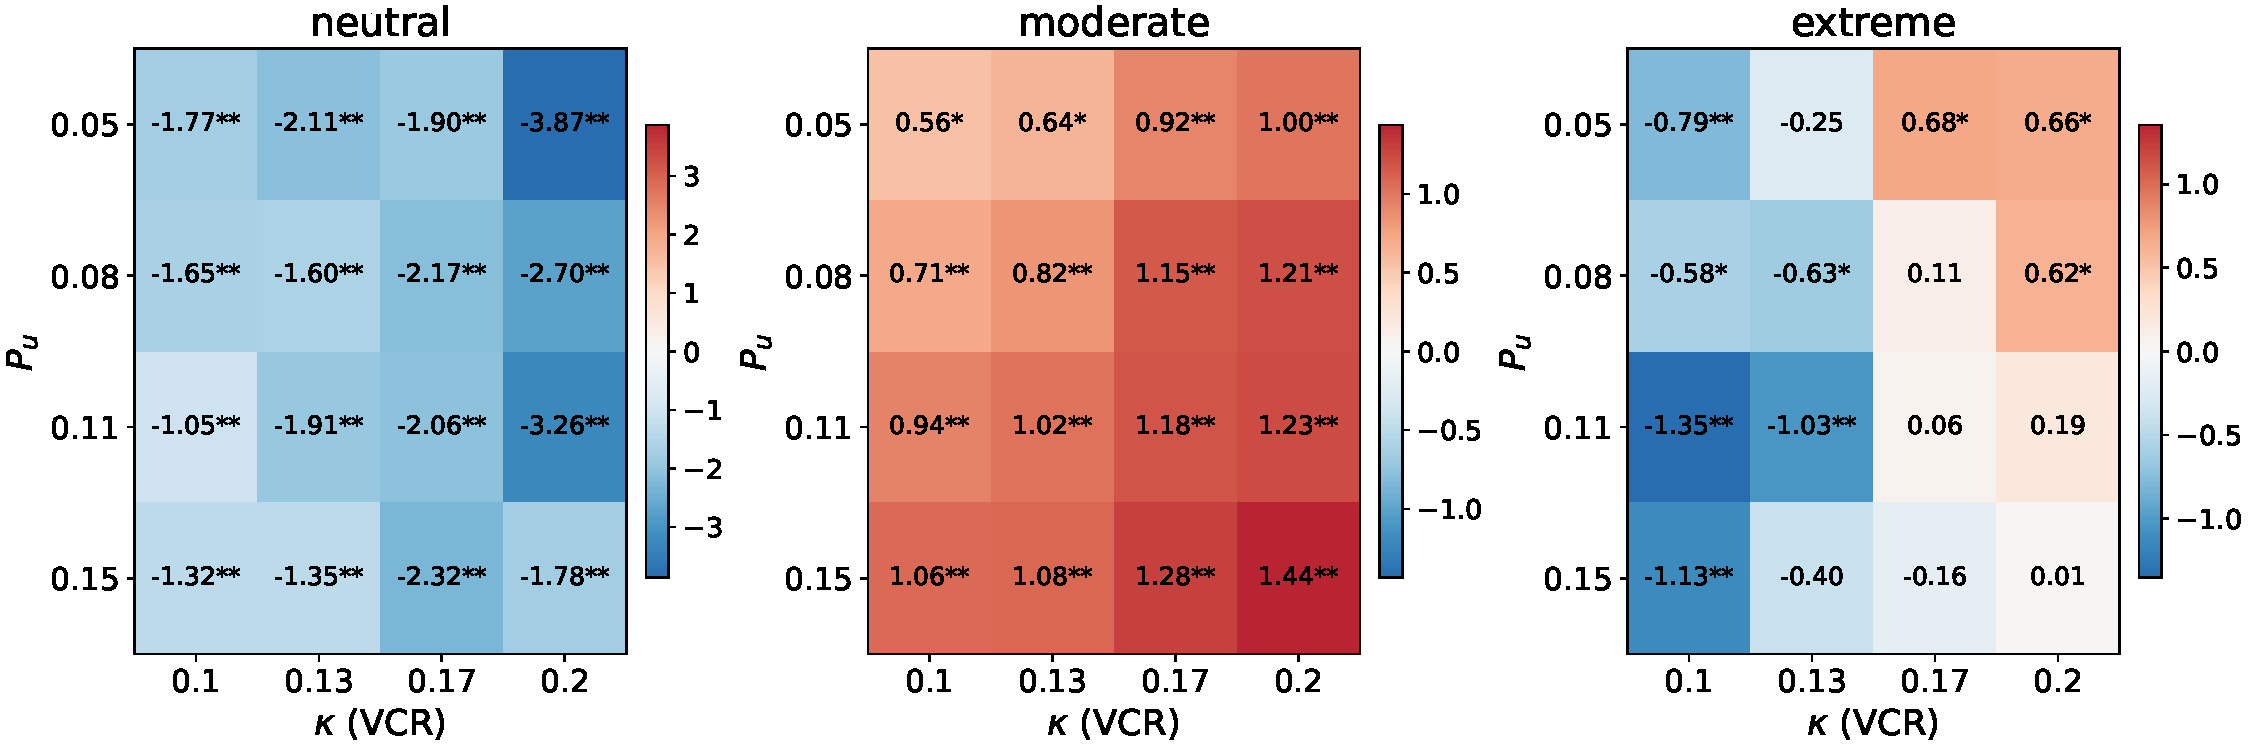
\includegraphics[width=\linewidth]{figures/outcome-heatmap.pdf}
\caption{Per-camp posting-rate effect size (Cohen's
$d$, M-silent minus control, paired per seed) across
the $P_u\times\VCR$ grid, for the moderate, near-extreme,
and extreme camps.}
\label{outcome-heatmap}
\end{figure}

Fig.~\ref{outcome-heatmap} shows heatmaps of the difference
in per-step per-capita posting counts for each of
the three opinion camps, averaged over steps
[39000, 40000], comparing \emph{M-silent} against
\emph{control}.
Steadily, the moderate camp boosts its posting
activity when it can perceive aligned-opinion
hubs' vocality, whereas the near-extreme camp
shrinks its posting by contrast.
Compared to these fairly intuitive results, the
extreme camp does not show a linear result: its
posting activity is reduced (a negative value in
the heatmap) when $\VCR$ is relatively low, for
each $P_u$ row, and it crosses the sign of its
effect at a different value of $\VCR$ depending on
the $P_u$ value.
Equivalently, reversing the contrast from
\emph{M-silent -- control} to \emph{control --
M-silent} lets us easily interpret the same difference
from the complementary perspective of the moderate
hub's activity rather than its absence. 
From this point of view, focusing on the presence
of moderate hubs, under the same propensity to
prune out-of-tolerance ties ($P_u$), moderate hubs
facilitate the extreme camp's posting activity
when agents speak only in the presence of
sufficient nearby agreement (low $\VCR$), and
mediate it in the opposite environment.

Also, $P_u$ can be interpreted as a modulator that
shifts the $\VCR$ cross-sign point, the watershed
value at which moderate hubs' vocality switches
between acting as a facilitator or a mediator for
the extreme camp.
In the extreme camp result of Fig.~\ref{outcome-heatmap},
the effect size in higher $P_u$ rows stays
negative across a wider range of low $\VCR$ before
turning positive at higher $\VCR$, compared with
lower $P_u$ rows.
This confirms that $P_u$ governs where this
regime shift occurs. 

Next, in order to see the upstream mechanism behind the
moderate hubs' cross-over role against extremes,
we investigated the interplay between near-extremes and
extremes.

\begin{figure}[t]
\centering
\includegraphics[width=\linewidth]{figures/NE-E-influx.pdf}
\caption{Converged, steady-state share of an extreme agent's feed
occupied by same-signed near-extreme-authored content, as a
percentage of that agent's actual, realized feed size -- which runs
well under the $\maxfeed$ capacity for the extreme camp -- across the
$P_u\times\VCR$ grid: for \emph{control} and \emph{M-silent}
separately (left, center), and their difference (right).}
\label{NE-E-influx}
\end{figure}

Fig.~\ref{NE-E-influx} shows, for every condition, the converged share
of an extreme agent's feed occupied by same-signed near-extreme-authored
content -- a population-averaged, steady-state feed-internal
proportion, not a per-step arrival count. We report this as a share of
the agent's actual, realized feed size rather than of the fixed
capacity $\maxfeed$, since an extreme agent's feed holds only a
handful of posts at any time (converged size $\approx$ 2--3 out of
$\maxfeed=15$): normalizing by capacity would understate the share
several-fold. This confirms that this share is steadily larger in
\emph{M-silent} conditions than in \emph{control} conditions.
This asymmetric influx difference between the two conditions,
shown in the rightmost panel, is mainly governed by $P_u$ and only
weakly by $\VCR$, growing several-fold as $P_u$ increases.

\section{Discussion}\label{sec:discussion}

The moderate and near-extreme camps -- whose posting activity
moderate-hub vocalization amplifies and suppresses, respectively, a
pattern confirmed uniformly in Fig.~\ref{outcome-heatmap} -- are
best understood together, since both effects follow from the same
single fact: posting probability, by construction
(Sec.~\ref{subsec:social-reinforcement}), depends on nothing other
than the fraction $c_i(t)$ of an agent's own feed that it currently
finds comfortable, so whichever camp's feed the moderate hubs' own
output reaches in substantial volume is the camp whose posting
behavior they move directly. The moderate camp is one such camp: a
moderate hub's opinion coincides with the moderate population's own
opinion range, so essentially every post that reaches a moderate
agent from a moderate hub falls within that agent's vocal comfort
radius $\VCR$. Moreover, moderate hubs supply the large majority of
the moderate-authored content the moderate population receives, so
silencing them drives a moderate agent's average feed-comfort
fraction from roughly $50\%$ down to roughly $30\%$, and its
posting activity down with it. The near-extreme camp is the second
such camp, but for the opposite reason. Moderate hubs occupy a
substantial share of a near-extreme agent's feed -- between roughly
a quarter and roughly a half, depending on $P_u$ -- but their
opinion is, relative to the narrow window $\VCR$, too far from the
near-extreme camp's own opinion range to register as comfortable.
Activating moderate hubs therefore dilutes a near-extreme agent's
comfort ratio and suppresses its posting, while silencing them
removes that dilution and reactivates it.

The extreme camp's own result, however, cannot be explained by
either of the two direct mechanisms above: a moderate hub's own
content never comes to occupy more than a few percent of an extreme
agent's feed, so the extreme camp's regime shift must be a
downstream, ripple consequence of something other than
moderate-hub content reaching extreme agents directly. We argue
that this something is the near-extreme-authored content flow:
specifically, how much of that flow reaches the extreme camp, and
how the arriving content is judged once it does, which are governed
by two further mechanisms operating in sequence -- an
\emph{openness} mechanism that determines how much near-extreme
content an extreme agent's feed admits, and a \emph{comfort}
mechanism that determines how much of what is admitted is judged
favorably.

The openness mechanism is governed by $P_u$, and it operates through
$\BoundedConfidence_i(t)$ rather than around it. Because a new
follow tie can only form, and an existing tie is only severed,
through $\BoundedConfidence_i(t)$, the width of an extreme agent's
own bounded-confidence threshold is what decides whether a
near-extreme author is eligible to be followed and retained, or is
instead blocked outright. Crucially, $\BoundedConfidence_i(t)$ does
not gate the near-extreme camp uniformly: since it is a distance
threshold and the near-extreme camp itself spans a range of
opinions between the extreme and moderate camps, a narrow
$\BoundedConfidence_i(t)$ admits only its \emph{extreme-ward} edge
while a wider $\BoundedConfidence_i(t)$ progressively extends
admission toward its \emph{moderate-ward} edge.
$\BoundedConfidence_i(t)$ therefore gates not only how much
near-extreme content is admitted, but how far into the near-extreme
range that admission reaches. We confirm, across every one of the
sixteen $P_u\times\VCR$ cells, that a higher $P_u$ is associated
with a wider converged $\BoundedConfidence_i(t)$ among extreme
agents, a monotonic trend (Kendall's $\tau=0.30$, $p<10^{-17}$,
$n=480$ pooled over all sixteen cells and seeds; $\tau=0.29$--$0.38$,
$p<10^{-4}$ within every individual $\VCR$ stratum) far too
consistent to be sampling noise. This pattern arises as follows:
$\BoundedConfidence_i$ is low in the opening steps regardless of
$P_u$, because agents are more likely to encounter out-of-tolerance
content before they have severed ties with such sources, and that
early exposure narrows $\BoundedConfidence_i$. From this low
starting point, agents gradually recover $\BoundedConfidence_i$ as
they finish unfollowing or blocking distant sources, and a higher
$P_u$ -- which prunes those sources faster -- lets that recovery
converge to a wider $\BoundedConfidence_i(t)$. Moreover, the
difference in near-extreme post volume reaching an extreme agent's
feed between the two conditions grows consistently with $P_u$,
supporting the \emph{openness} role of $P_u$: it is
$\BoundedConfidence_i$ that gates how much near-extreme content an
extreme agent admits.

The comfort mechanism, by contrast, is governed by $\VCR$ alone,
independent of $P_u$. Whatever near-extreme content the openness
mechanism admits, $\VCR$ then determines the evaluation of that
content: comfortable if within $\VCR$, uncomfortable otherwise.
$\VCR$ is therefore what fixes the \emph{sign} of the extreme
camp's regime shift: under a narrow $\VCR$, almost none of the
admitted near-extreme content falls inside the comfort range, so
admission only dilutes the comfort ratio and posting moves
downward; under a wide $\VCR$, a non-trivial share does fall inside
the comfort range, so posting moves upward instead. In other words,
under the same $P_u$, silencing moderate hubs deactivates extreme
posting when $\VCR$ is low, and activates it when $\VCR$ is high; we
refer to the $\VCR$ value at which the effect crosses zero as its
\emph{sign-change point}. As shown in Fig.~\ref{outcome-heatmap},
this sign-change point shifts toward higher $\VCR$ as $P_u$
increases, because the wider $\BoundedConfidence_i(t)$ that higher
$P_u$ produces retains near-extreme sources whose opinion sits
closer to the moderate end of that camp, so a wider $\VCR$ is
needed before their content registers as comfortable. Notably, the
effect is relatively small at high $\VCR$ and high $P_u$ in
Fig.~\ref{outcome-heatmap}: the wider $\BoundedConfidence_i$ that
high $P_u$ produces admits more comfortable near-extreme content,
but more uncomfortable near-extreme content alongside it, so the
two increases partly cancel and the net difference between
conditions shrinks.

To capture the effect of an \emph{active} moderate hub specifically,
we restate the mechanism above from its own perspective,
complementary to the silencing account so far. The negative region
of Fig.~\ref{outcome-heatmap} is the facilitating regime, where an
active moderate hub boosts extreme posting; the positive region is
the suppressing regime, where it suppresses extreme posting. In the
facilitating regime ($\VCR$ low), the disruptive near-extreme
content that would otherwise arrive under \emph{M-silent} simply
does not arrive, so the extreme camp's feed stays comfortable. In
the suppressing regime ($\VCR$ high), it is instead the near-extreme
content that $\BoundedConfidence_i(t)$ would have admitted -- on
the near-extreme camp's extreme-ward edge, close enough to also
satisfy $\VCR$ -- that fails to arrive, so the extreme camp loses a
source of comfortable content it would otherwise have had. An
active moderate hub therefore acts less as a conduit than as an
upstream regulator: $\BoundedConfidence_i$ determines what
near-extreme content can reach the extreme camp, while $\VCR$
determines whether the excluded content would have been welcome or
unwelcome.

\section{Conclusion}\label{sec:conclusion}
Although the separation by fifth bins with agents' opinions 
degenerate this continuous ripple-ish effect, this formalization 
sufficiently gives us the implication of counter-intuitive 
effect by moderate hubs' vocality. -> as a limitation and 
hint for further reserach.

\bibliographystyle{spmpsci}
\bibliography{refs}
\end{document}
